\section{Implicit Finite Volume Method for Incompressible Flows -- Fully Coupled Approach}
\label{sec:cpld}

Since the antecedent section \ref{sec:seg} already discussed the discretization details on the involved equations, this section aims at a comparison at the algorithmic level of the SIMPLE algorithm, presented in section \ref{sec:simple}, as a method to resolve the pressure-velocity coupling, and an implementation of a fully coupled solution algorithm. It should be noted that the discretization of the equations to be solved is not changed in any way to maintain comparability, so the presented differences are exclusively due to difference in the solution algorithm. Successful implementations of a fully coupled solution algorithm for incompressible Navier-Stokes equations have been presented in \cite{chen10,darwish09,falk13,vakilipour12}. In addition the presented work will extend the solution approach presented in \cite{falk13} to three-dimensional domains. Furthermore this section will present various approaches to incorporate different degrees of velocity-to-temperature and temperature-to-velocity/pressure coupling. Finally the structure of the resulting linear system to be solved is discussed.

\subsection{The Fully Coupled Algorithm -- Pressure-Velocity Coupling Revised}

This subsection motivates the use of a fully coupled algorithm to resolve pressure-velocity coupling and mentions the differences to the approach presented in subsection \ref{sec:simple}. The mentioned subsection presented a common solution approach to solve incompressible Navier-Stokes equations: After the linearization of the equations, momentum balances were solved using the pressure from the previous iteration as a guess. Since in general the velocity field obtained by solving a momentum balance with a guessed pressure does not obey continuity, the velocity field and the pressure field had to be corrected. This in turn would lead to an inferior solution regarding the residual of the momentum balances. To avoid this iterative guess-and-correct solution process another class of approaches to the pressure-velocity coupling problematic, represented by algorithms that are \emph{fully coupled}, will be introduced now. . 

The central aspect of fully coupled solution methods for Navier-Stokes equations is, that instead of solving for the velocities and pressure corrections sequentially, the velocity field and the pressure are solved for simultaneously \cite{schaefer99}, so every velocity field that is calculated obeys conservation of momentum and mass, without the need to be corrected. As a result the under-relaxation of pressure and velocities is no longer required, which accelerates convergence significantly in terms of needed outer iterations. The only reason for still needing an iterative solution process is the non-linearity of the Navier-Stokes equations which is accounted for by the use of the Picard iteration process, which has been presented in subsection \ref{sec:nonlinear}. The iterations fortunately make room for deferred corrections as introduced in subsection \ref{sec:segdiscretization}. It should be noted that it is also possible to use the coupled solution algorithm to calculate pressure corrections. Reference \cite{klaij13} uses this approach to solve the Navier-Stokes equations.

On the downside implementations of fully coupled solution methods require significantly more system memory than segregated methods. This is due to the higher amount of information that has to be available at the same time and the resulting linear systems which also require more memory, due to the increased amount of unknowns to solve for. Furthermore the bad condition of the linear algebraic system \cite{schaefer99} tends to slow down the convergence of the equation solver algorithm.

As in the case of segregated methods it is not advisable to solve the mass balance equation directly \cite{schaefer99}. Instead of deriving an equation for the pressure correction \(p'\), as shown in \ref{sec:simple}, an equation for the pressure is derived by using the pressure-weighted interpolation method, which has been introduced in \ref{sec:massflux} and is used to approximate the velocities in the discretized mass balance (\ref{eq:massbalance}). Concretely equation (\ref{eq:pwim}) is adapted for the use in a fully coupled algorithm
\begin{displaymath}
  u_{i,f}^{(n)} 
  =
  \left[\left(1 - \gamma_f\right) u_{i,P}^{(n)} + \gamma_f u_{i,Q}^{(n)} \right]
  - \left(\left(1 - \gamma_f\right) \frac{V_P}{a_P^{u_i}} + \gamma_f \frac{ V_Q}{a_Q^{u_i}}\right)
  \left[ 
    \underline{ \left(\frac{\partial p}{\partial x_i}\right)_f^{(n)}}
  - \frac{1}{2} 
  \left( 
    \left( \frac{\partial p}{\partial x_i} \right)_P^{(n-1)} 
  + \left(\frac{\partial p}{\partial x_i}\right)_Q^{(n-1)} 
  \right)
  \right].
\end{displaymath}
The changes comprise the removal of last term of (\ref{eq:pwim}) accounting for the under-relaxation, since no under-relaxation is needed in fully coupled algorithms which is equivalent to an under-relaxation factor \(\alpha_\vec{u} = 1\). Furthermore the underlined partial derivatives are now going to be treated implicitly. This leads to the semi-implicit pressure equation
\begin{align}
  \sum_{F \in NB(P)} 
  \rho
  \left[\left(1 - \gamma_f\right) u_{i,P}^{(n)} + \gamma_f u_{i,F}^{(n)} \right]\,  S_f
  - \rho \left(\left(1 - \gamma_f\right) \frac{ V_P}{a_P^{u_i}} + \gamma_f \frac{ V_F}{a_F^{u_i}}\right)
  \left[ 
  \left(\frac{\partial p}{\partial x_i}\right)_f^{(n)}
  \right]\,  S_f \nonumber \\
  =
  - \sum_{F \in NB(P)}
  \rho
  \left(\left(1 - \gamma_f\right) \frac{ V_P}{a_P^{u_i}} + \gamma_f \frac{ V_F}{a_F^{u_i}}\right)
  \left[ 
  \frac{1}{2} 
  \left( 
    \left( \frac{\partial p}{\partial x_i} \right)_P^{(n-1)} 
  + \left(\frac{\partial p}{\partial x_i}\right)_F^{(n-1)} 
  \right)
  \right] \, S_f.
\end{align}

Even though this equation is solved for the pressure \(p\) while equation (\ref{eq:presscorr}) is solved for the pressure correction \(p'\) the matrix coefficients from the pressure correction discretization of equation (\ref{eq:segpresscorrcoeff}) and the calculation of the right hand side is given in equation (\ref{eq:presscorrb}). For the implicit coupling to the velocities \(u_i\) additional matrix coefficients have to be considered. These can be calculated as
\begin{displaymath}
  a_F^{p,u_i} = \rho \, \gamma_f S_f \quad \text{and} \quad a_P^{p,u_i} = \sum_{F \in NB(P)} \rho \, (1-\gamma_f) \, S_f.
\end{displaymath}

On the other side the discretized momentum balance gives matrix coefficients to account for the implicit velocity-pressure coupling. They are calculated as
\begin{displaymath}
  a_F^{u_i,p} =  \gamma_f S_f \quad \text{and} \quad a_P^{u_i,p} = \sum_{F \in NB(P)} (1-\gamma_f) \, S_f.
\end{displaymath}
If the Boussinesq approximation is used implicitly, an additional coefficient \(a_P^{u_i,T}\) to account for the velocity temperature coupling has to be considered. This will be handled in subsection \ref{sec:temperaturecoupling}

\alglanguage{pseudocode}
\begin{algorithm}
\label{al:coupled}
\caption{Fully Coupled Solution Algorithm}
\begin{algorithmic}
\State{\textit{INITIALIZE} variables}
\While{(convergence criterion not accomplished)}
\If{(temperature coupling)}
  \State{\textit{SOLVE} the linear system for velocities, pressure and temperature}
\Else
  \State{\textit{SOLVE} the linear system for velocities and pressure}
\EndIf
\State{\textit{CALCULATE} mass fluxes using REFERENCE}
\If{(decoupled scalar equation)}
  \State{\textit{SOLVE} scalar equation as described in \textbf{(\ref{sec:discretetemperature})}}
\EndIf
\EndWhile
\end{algorithmic}
\end{algorithm}

\subsection{Coupling to the Temperature Equation}
\label{sec:temperaturecoupling}

Since the present work also aims at analyzing the efficiency of different methods to couple the temperature equation to the velocities and vice-versa this subsection discusses different approaches to handle the coupling of the temperature equation to the Navier-Stokes equations if the Boussinesq-Approximation, as introduced in subsection \ref{sec:boussinesq}, is used. The effectiveness of realizing a strong coupling of the temperature equation to the Navier-Stokes equations depends on the flow problem. The physical coupling tends to increase in flow scenarios of natural convection, where the temperature difference and hence the buoyancy term in the Navier-Stokes equations dominates the fluid movement. Generally speaking: The higher the physical coupling of temperature and flow, the greater are the benefits of using an implementation that uses a strong coupling to the temperature equation. The following subsections present different approaches that can be used for different intensities of coupling.
      
\subsubsection{Decoupled Approach -- Explicit Velocity-to-Temperature Coupling}

The decoupled approach is similar to the treatment of the velocity-temperature coupling described in subsection \ref{sec:segdiscretization}. If this approach is chosen no special measures have to be taken. The momentum balances receive a contribution \( b_P^{u_i,T}\) with
\begin{displaymath}
  b_P^{u_i,T} := - \rho \beta \left( T_P^{(n-1)} - T_0 \right) V_P,
\end{displaymath}
that handles the coupling explicitly by using the temperature result of the previous outer iteration. In some cases it might be necessary to under-relax the temperature each iteration

\subsubsection{Implicit Velocity-to-Temperature Coupling}

In the same way it is possible to realize the coupling described in the previous subsection by implicitly considering the temperature in the momentum balances, which leads to an additional matrix coefficient \(a_P^{u_i,T}\) and an additional contribution to the right hand side accounting for the coupling to the temperature equation
\begin{displaymath}
  a_P^{u_i,T} = \rho \beta V_P 
  \quad \text{and} \quad
  b_P^{u_i,T} = \rho \beta T_0 V_P.
\end{displaymath}

\subsubsection{Temperature-to-Velocity/Pressure Coupling -- Newton-Raphson Linearization}

The previous section discussed the velocity temperature coupling and so far only the momentum balances were affected by the realization of the coupling methods. Independently it is possible to couple the temperature equation not only to the momentum balances but also to the pressure equation. In section \ref{sec:discretetemperature} the non-linear partial differential equation was linearized using a Picard iteration method. Specifically the convective term \(\rho u_j T\) was linearized by taking the mass flux from the antecedent solve of the momentum and pressure correction equations. If the decoupled approach is used, this treatment remains valid. But, if an implicit temperature coupling is sought, a coupling of the temperature equation to the momentum balances which considers the mass fluxes is desirable. Methods that exhibit the described property can be found in \cite{galpin86,oliveira01,sheu04,vakilipour12}. A common denomination of the therein used linearization method is called \emph{Newton-Raphson linearization} which can be interpreted as a bilinear approximation of the convective term by the linear terms of the respective Taylor polynomial.

The Newton-Raphson linearization technique is applied to the convective term of the temperature equation as follows. A first order Taylor approximation of the the mass specific convective flux through the boundary face \(S_f\) around the \(n-1\)nt iteration value yields for the approximation at the \(n\)th iteration
\begin{align*}
  \left(u_{j,f} T_f \right)^{(n)} 
  &\approx 
  \left(u_{j,f} T_f \right)^{(n-1)} 
  + \frac{\partial}{\partial u_{j,f}}\left( u_{j,f} T_f \right)^{(n-1)} \left(u_{j,f}^{(n)} - u_{j,f}^{(n-1)} \right) 
  + \frac{\partial}{\partial T_f}\left( u_{j,f} T_f \right)^{(n-1)} \left( T_f^{(n)} - T_f^{(n-1)} \right) \\[0.5em]
  &=
  (u_{j,f} T_f )^{(n-1)} 
  + \vphantom{(u_{j,f} T_f)}{T_f}^{(n-1)} (\vphantom{(u_{j,f} T_f)}{u_{j,f}}^{(n)} - \vphantom{(u_{j,f} T_f)}{u_{j,f}}^{(n-1)} ) 
  +  \vphantom{(u_j T)}{u_{j,f}}^{(n-1)} ( \vphantom{(u_j T)}{T_f}^{(n)} - \vphantom{(u_j T)}{T_f}^{(n-1)} ) \\[0.7em]
  &=
  \underline{\vphantom{(u_j T)}{u_{j,f}}^{(n-1)} \vphantom{(u_{j,f})}{T_f}^{(n)}}  + \vphantom{(u_{j,f} T_f)}{u_{j,f}}^{(n)} \vphantom{(u_jT)}{T_f}^{(n-1)}  -  \vphantom{(u_j T)}{u_{j,f}}^{(n-1)} \vphantom{(u_j T)}{T_f}^{(n-1)}.
\end{align*}
A comparison with section \ref{sec:segconvective} shows, that the underlined term coincides with the term from the usual linearization. The first of the two new terms will be treated implicitly and explicitly after using the pressure-weighted interpolation method from section \ref{sec:pwim} to interpolate the value of \(u_{j,f}\). The second term will be treated explicitly. The use of the pressure-weighted interpolation method does not only create a temperature-to-velocity but also a temperature-to-pressure coupling. Applying the pressure-weighted interpolation, the equation for the mass specific convective flux reads
\begin{align*}
  \left(u_{j,f} T_f \right)^{(n)} 
  &\approx 
  \underline{\vphantom{(u_j T)}{u_{j,f}}^{(n-1)} \vphantom{(u_{j,f})}{T_f}^{(n)}} + \vphantom{(u_jT)}{T_f}^{(n-1)}  \left[\left(1 - \gamma_f\right) u_{j,P}^{(n)} + \gamma_f u_{j,Q}^{(n)} \right] \nonumber\\[1em]
    &\quad\quad 
    - T_f^{(n-1)}\left(\left(1 - \gamma_f\right) \frac{\alpha_\vec{u} V_P}{a_P^{u_j}} + \gamma_f \frac{\alpha_\vec{u} V_Q}{a_Q^{u_j}}\right)
    \left[ 
    \left(\frac{\partial p}{\partial x_j}\right)_f^{(n)} 
    -  \frac{1}{2} \left( \frac{\partial p}{\partial x_j} \right)_P^{(n-1)} 
    - \frac{1}{2} \left(\frac{\partial p}{\partial x_j}\right)_Q^{(n-1)} 
    \right] \nonumber \\[1em]
    &  \quad\quad -\vphantom{(u_j T)}{u_{j,f}}^{(n-1)} \vphantom{(u_j T)}{T_f}^{(n-1)}.
\end{align*}
If this semi-implicit, semi-discrete equation is discretized completely new matrix and contributions can be calculated
\begin{align*}
  \allowdisplaybreaks
  &a_F^{T,u_i} = \rho T_f^{(n-1)} \gamma_f n_{f,i} S_f \\[1.0em] 
  &a_P^{T,u_i} = \sum_{F \in NB(P)} \rho T_f^{(n-1)} \left(1-\gamma_f\right) n_{f,i} S_f \\[1.0em]
  &a_F^{T,p} = -\rho T_f^{(n-1)} \left(\left(1 - \gamma_f\right) \frac{\alpha_\vec{u} V_P}{a_P^{u_i}} + \gamma_f \frac{\alpha_\vec{u} V_F}{a_F^{u_i}}\right) \frac{S_f}{\left(\vec{x}_P - \vec{x}_F\right) \cdot \vec{n}_f} = \rho T_f^{(n-1)} a_F^{p} \\[1.0em] 
  &\text{and} \quad
  a_P^{T,p} = - \sum_{F \in NB(P)} T_f^{(n-1)} a_F^{T,p}.
\end{align*}
The explicit parts resulting from the Newton-Raphson linearization result in additional contributions to the right hand side

\subsection{Boundary Conditions on Domain and Block Boundaries}

\subsubsection{Dirichlet Boundary Condition for Velocity}

Mention that the Newton-Raphson linearization is not considered on Dirichlet boundaries.

%\subsubsection{Dirichlet Boundary Condition for Pressure} NOT TO BE USED

\subsubsection{Wall Boundary Condition}

\subsubsection{Block Boundary Condition}

\subsection{Assembly of Linear Systems -- Final Form of Equations}

\begin{figure}
  \centering
  \label{fig:segassemble}
  
\newcommand*{\xMin}{0}%
\newcommand*{\xMax}{12}%
\newcommand*{\xStep}{1.5}%
\newcommand*{\nStep}{5}
\newcommand*{\yMin}{0}%
\newcommand*{\yMax}{1}%
\newcommand\markcell[3] {
  \fill[gray,draw=black] (#2*\xStep,\xStep*\nStep-#1*\xStep) -- (#2*\xStep+\xStep,\xStep*\nStep-#1*\xStep) -- (#2*\xStep+\xStep,\xStep*\nStep-#1*\xStep-\xStep) -- (#2*\xStep,\xStep*\nStep-#1*\xStep-\xStep) -- cycle;
  \node[anchor=center,font=\large] at (#2*\xStep+0.5*\xStep,\xStep*\nStep-#1*\xStep-0.5*\xStep) {#3};
  }

\newcommand\markcellblue[3] {
  \fill[cyan,draw=black] (#2*\xStep,\xStep*\nStep-#1*\xStep) -- (#2*\xStep+\xStep,\xStep*\nStep-#1*\xStep) -- (#2*\xStep+\xStep,\xStep*\nStep-#1*\xStep-\xStep) -- (#2*\xStep,\xStep*\nStep-#1*\xStep-\xStep) -- cycle;
  \node[anchor=center,font=\large] at (#2*\xStep+0.5*\xStep,\xStep*\nStep-#1*\xStep-0.5*\xStep) {#3};
  }

\newcommand\markcellred[3] {
  \fill[red,draw=black] (#2*\xStep,\xStep*\nStep-#1*\xStep) -- (#2*\xStep+\xStep,\xStep*\nStep-#1*\xStep) -- (#2*\xStep+\xStep,\xStep*\nStep-#1*\xStep-\xStep) -- (#2*\xStep,\xStep*\nStep-#1*\xStep-\xStep) -- cycle;
  \node[anchor=center,font=\large] at (#2*\xStep+0.5*\xStep,\xStep*\nStep-#1*\xStep-0.5*\xStep) {#3};
  }

\newcommand\markcellgreen[3] {
  \fill[green,draw=black] (#2*\xStep,\xStep*\nStep-#1*\xStep) -- (#2*\xStep+\xStep,\xStep*\nStep-#1*\xStep) -- (#2*\xStep+\xStep,\xStep*\nStep-#1*\xStep-\xStep) -- (#2*\xStep,\xStep*\nStep-#1*\xStep-\xStep) -- cycle;
  \node[anchor=center,font=\large] at (#2*\xStep+0.5*\xStep,\xStep*\nStep-#1*\xStep-0.5*\xStep) {#3};
  }

\newcommand*{\xStepp}{0.15}%
\newcommand*{\nStepp}{35}
\newcommand*{\offset}{5}
\newcommand\markcelll[3] {
  \fill[gray,draw=black] (#2*\xStepp-\offset,\xStepp*\nStepp-#1*\xStepp-\offset) -- (#2*\xStepp+\xStepp-\offset,\xStepp*\nStepp-#1*\xStepp-\offset) -- (#2*\xStepp+\xStepp-\offset,\xStepp*\nStepp-#1*\xStepp-\xStepp-\offset) -- (#2*\xStepp-\offset,\xStepp*\nStepp-#1*\xStepp-\xStepp-\offset) -- cycle;
  }

\newcommand\markcellbluee[3] {
  \fill[orange,draw=black] (#2*\xStepp-\offset,\xStepp*\nStepp-#1*\xStepp-\offset) -- (#2*\xStepp+\xStepp-\offset,\xStepp*\nStepp-#1*\xStepp-\offset) -- (#2*\xStepp+\xStepp-\offset,\xStepp*\nStepp-#1*\xStepp-\xStepp-\offset) -- (#2*\xStepp-\offset,\xStepp*\nStepp-#1*\xStepp-\xStepp-\offset) -- cycle;
  }

\newcommand\markcellblackk[3] {
  \fill[black,draw=black] (#2*\xStepp-\offset,\xStepp*\nStepp-#1*\xStepp-\offset) -- (#2*\xStepp+\xStepp-\offset,\xStepp*\nStepp-#1*\xStepp-\offset) -- (#2*\xStepp+\xStepp-\offset,\xStepp*\nStepp-#1*\xStepp-\xStepp-\offset) -- (#2*\xStepp-\offset,\xStepp*\nStepp-#1*\xStepp-\xStepp-\offset) -- cycle;
  }

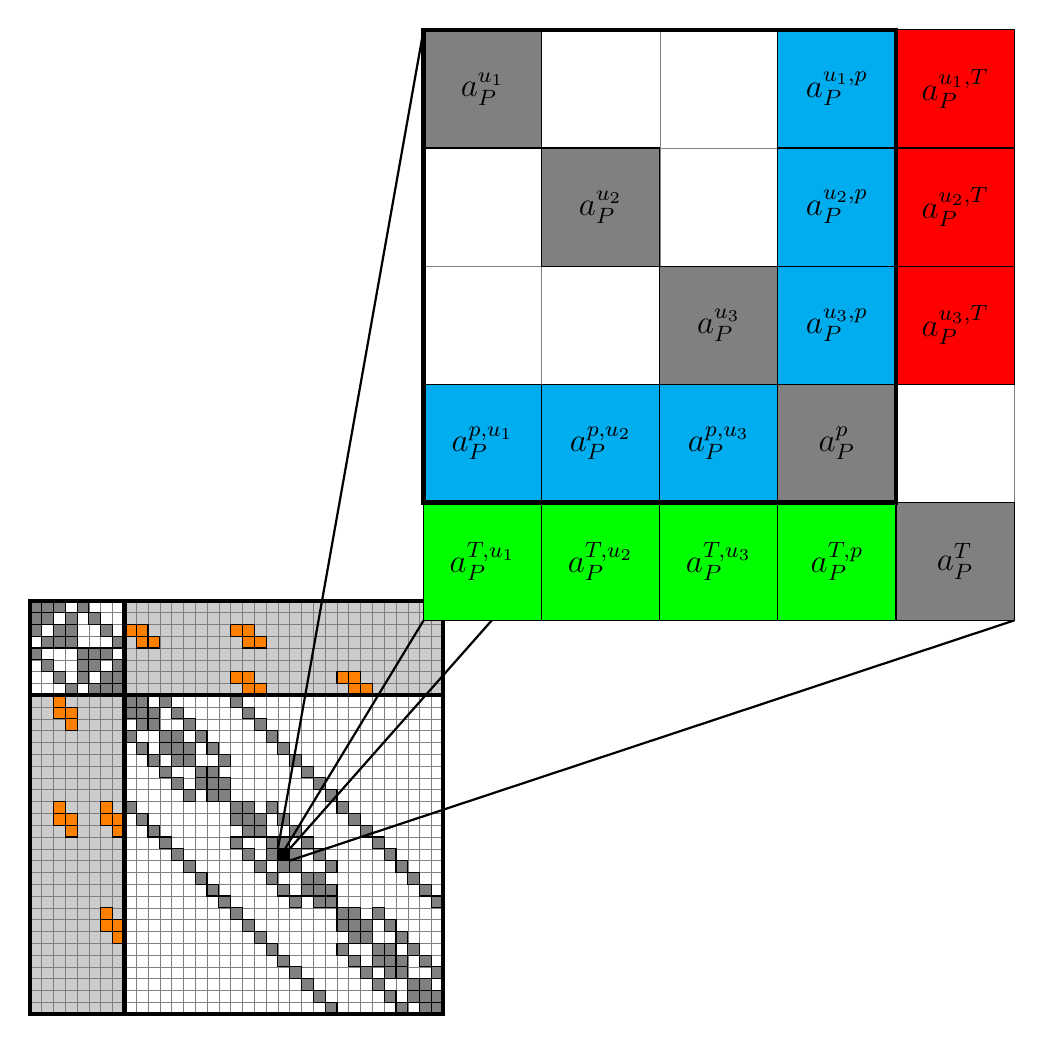
\begin{tikzpicture}


    %SMALL MATRIX%%%%%%%%%%%%%%%%%%%%%%%%%%%%%%%%%%%%%%%%%%%%%%%%%%%%%%%%%%%%%%%%%%%%%%%%%%%%%%%%%%%%%%%%%%%%%%%%%%%%%%%%%%%%%%%%%%
    %BACKGROUND COLORING
    \fill[gray!40] (0-\offset,\xStepp*\nStepp-8*\xStepp-\offset) -- (8*\xStepp-\offset,\xStepp*\nStepp-8*\xStepp-\offset) -- (8*\xStepp-\offset,0-\offset) -- (0*\xStepp-\offset,0-\offset) -- cycle;
    \fill[gray!40] (8*\xStepp-\offset,\xStepp*\nStepp-\offset) -- (35*\xStepp-\offset,\xStepp*\nStepp-\offset) -- (35*\xStepp-\offset,\xStepp*\nStepp-\offset-8*\xStepp) -- (8*\xStepp-\offset,\xStepp*\nStepp-8*\xStepp-\offset) -- cycle;

    \foreach \j in {0,...,35} {
        \draw [very thin,gray] (0-\offset,\j*\xStepp-\offset) -- (\xStepp*\nStepp-\offset,\j*\xStepp-\offset)  ;
        \draw [very thin,gray] (\j*\xStepp-\offset,0-\offset) -- (\j*\xStepp-\offset,\xStepp*\nStepp-\offset)  ;
    }

    \foreach \i in {0,...,34} {
      \markcelll {\i}{\i}{};
    }

    %BLOCK 1
    \markcelll {0}{1}{};
    \markcelll {0}{2}{};
    \markcelll {0}{4}{};

    \markcelll {1}{0}{};
    \markcelll {1}{3}{};
    \markcelll {1}{5}{};

    \markcelll {2}{3}{};
    \markcelll {2}{0}{};
    \markcelll {2}{6}{};

    \markcelll {3}{2}{};
    \markcelll {3}{1}{};
    \markcelll {3}{7}{};

    \markcelll {4}{5}{};
    \markcelll {4}{6}{};
    \markcelll {4}{0}{};

    \markcelll {5}{4}{};
    \markcelll {5}{7}{};
    \markcelll {5}{1}{};

    \markcelll {6}{7}{};
    \markcelll {6}{4}{};
    \markcelll {6}{2}{};

    \markcelll {7}{6}{};
    \markcelll {7}{5}{};
    \markcelll {7}{3}{};
     
    %BLOCK2
    \markcelll {8 }{9 }{};
    \markcelll {8 }{11}{};
    \markcelll {8 }{17}{};

    \markcelll {9 }{8 }{};
    \markcelll {9 }{10}{};
    \markcelll {9 }{12}{};
    \markcelll {9 }{18}{};

    \markcelll {10}{9 }{};
    \markcelll {10}{13}{};
    \markcelll {10}{19}{};

    \markcelll {11}{8 }{};
    \markcelll {11}{12}{};
    \markcelll {11}{14}{};
    \markcelll {11}{20}{};

    \markcelll {12 }{9 }{};
    \markcelll {12 }{11}{};
    \markcelll {12 }{13}{};
    \markcelll {12 }{15}{};
    \markcelll {12 }{21}{};

    \markcelll {13}{10}{};
    \markcelll {13}{12}{};
    \markcelll {13}{16}{};
    \markcelll {13}{22}{};

    \markcelll {14}{11}{};
    \markcelll {14}{15}{};
    \markcelll {14}{23}{};

    \markcelll {15 }{12}{};
    \markcelll {15 }{14}{};
    \markcelll {15 }{16}{};
    \markcelll {15 }{24}{};

    \markcelll {16}{13}{};
    \markcelll {16}{15}{};
    \markcelll {16}{25}{};

    \markcelll {17}{18 }{};
    \markcelll {17}{20}{};
    \markcelll {17}{26}{};
    \markcelll {17}{8 }{};

    \markcelll {18}{17}{};
    \markcelll {18}{19}{};
    \markcelll {18}{21}{};
    \markcelll {18}{27}{};
    \markcelll {18}{9 }{};

    \markcelll {19}{18}{};
    \markcelll {19}{22}{};
    \markcelll {19}{28}{};
    \markcelll {19}{10}{};

    \markcelll {20}{17}{};
    \markcelll {20}{21}{};
    \markcelll {20}{23}{};
    \markcelll {20}{29}{};
    \markcelll {20}{11}{};

    \markcelll {21}{18}{};
    \markcelll {21}{20}{};
    \markcelll {21}{22}{};
    \markcelll {21}{24}{};
    \markcelll {21}{30}{};
    \markcelll {21}{12}{};

    \markcelll {22}{19}{};
    \markcelll {22}{21}{};
    \markcelll {22}{25}{};
    \markcelll {22}{31}{};
    \markcelll {22}{13}{};

    \markcelll {23}{20}{};
    \markcelll {23}{24}{};
    \markcelll {23}{32}{};
    \markcelll {23}{14}{};

    \markcelll {24}{21}{};
    \markcelll {24}{23}{};
    \markcelll {24}{25}{};
    \markcelll {24}{33}{};
    \markcelll {24}{15}{};

    \markcelll {25}{22}{};
    \markcelll {25}{24}{};
    \markcelll {25}{34}{};
    \markcelll {25}{16}{};



    \markcelll {26}{27}{};
    \markcelll {26}{29}{};
    \markcelll {26}{17}{};

    \markcelll {27}{26}{};
    \markcelll {27}{28}{};
    \markcelll {27}{30}{};
    \markcelll {27}{18}{};

    \markcelll {28}{27}{};
    \markcelll {28}{31}{};
    \markcelll {28}{19}{};

    \markcelll {29}{26}{};
    \markcelll {29}{30}{};
    \markcelll {29}{32}{};
    \markcelll {29}{20}{};

    \markcelll {30}{27}{};
    \markcelll {30}{29}{};
    \markcelll {30}{31}{};
    \markcelll {30}{33}{};
    \markcelll {30}{21}{};

    \markcelll {31}{28}{};
    \markcelll {31}{30}{};
    \markcelll {31}{34}{};
    \markcelll {31}{22}{};

    \markcelll {32}{29}{};
    \markcelll {32}{33}{};
    \markcelll {32}{23}{};

    \markcelll {33}{30}{};
    \markcelll {33}{32}{};
    \markcelll {33}{34}{};
    \markcelll {33}{24}{};

    \markcelll {34}{31}{};
    \markcelll {34}{33}{};
    \markcelll {34}{25}{};

    %Connectivities
    \markcellbluee {2}{8}{};
    \markcellbluee {2}{9}{};
    \markcellbluee {2}{17}{};
    \markcellbluee {2}{18}{};

    \markcellbluee {3}{9}{};
    \markcellbluee {3}{10}{};
    \markcellbluee {3}{18}{};
    \markcellbluee {3}{19}{};

    \markcellbluee {6}{17}{};
    \markcellbluee {6}{18}{};
    \markcellbluee {6}{26}{};
    \markcellbluee {6}{27}{};

    \markcellbluee {7}{18}{};
    \markcellbluee {7}{19}{};
    \markcellbluee {7}{27}{};
    \markcellbluee {7}{28}{};

    \markcellbluee {8}{2}{};
    \markcellbluee {9}{2}{};
    \markcellbluee {17}{2}{};
    \markcellbluee {18}{2}{};

    \markcellbluee {9}{3}{};
    \markcellbluee {10}{3}{};
    \markcellbluee {18}{3}{};
    \markcellbluee {19}{3}{};

    \markcellbluee {17}{6}{};
    \markcellbluee {18}{6}{};
    \markcellbluee {26}{6}{};
    \markcellbluee {27}{6}{};

    \markcellbluee {18}{7}{};
    \markcellbluee {19}{7}{};
    \markcellbluee {27}{7}{};
    \markcellbluee {28}{7}{};

    \draw[ultra thick] (0-\offset,\xStepp*\nStepp-\offset) -- (8*\xStepp-\offset,\xStepp*\nStepp-\offset) -- (8*\xStepp-\offset,\xStepp*\nStepp-8*\xStepp-\offset) -- (0-\offset,\xStepp*\nStepp-8*\xStepp-\offset) -- cycle;
    \draw[ultra thick] (8*\xStepp-\offset,\xStepp*\nStepp-\offset) -- (35*\xStepp-\offset,\xStepp*\nStepp-\offset) -- (35*\xStepp-\offset,\xStepp*\nStepp-8*\xStepp-\offset) -- (8*\xStepp-\offset,\xStepp*\nStepp-8*\xStepp-\offset) -- cycle;
    \draw[ultra thick] (8*\xStepp-\offset,\xStepp*\nStepp-8*\xStepp-\offset) -- (35*\xStepp-\offset,\xStepp*\nStepp-8*\xStepp-\offset) -- (35*\xStepp-\offset,0-\offset) -- (8*\xStepp-\offset,0-\offset) -- cycle;
    \draw[ultra thick] (0-\offset,\xStepp*\nStepp-8*\xStepp-\offset) -- (8*\xStepp-\offset,\xStepp*\nStepp-8*\xStepp-\offset) -- (8*\xStepp-\offset,0-\offset) -- (0*\xStepp-\offset,0-\offset) -- cycle;

    \coordinate (A1) at (21*\xStepp-\offset,\xStepp*\nStepp-21*\xStepp-\offset);
    \coordinate (A2) at (21*\xStepp+\xStepp-\offset,\xStepp*\nStepp-21*\xStepp-\offset);
    \coordinate (A3) at (21*\xStepp+\xStepp-\offset,\xStepp*\nStepp-21*\xStepp-\xStepp-\offset);
    \coordinate (A4) at (21*\xStepp-\offset,\xStepp*\nStepp-21*\xStepp-\xStepp-\offset);
    \markcellblackk {21}{21}{};

    %\draw[fill=black] (A1) circle (0.15em);
    %\draw[fill=black] (A2) circle (0.15em);
    %\draw[fill=black] (A3) circle (0.15em);
    %\draw[fill=black] (A4) circle (0.15em);

    \draw[thick] (A1) -- (0,7.5);
    \draw[thick] (A2) -- (7.5,7.5);
    \draw[thick] (A3) -- (7.5,0);
    \draw[thick] (A4) -- (0,0);

    %CPLD MATRIX%%%%%%%%%%%%%%%%%%%%%%%%%%%%%%%%%%%%%%%%%%%%%%%%%%%%%%%%%%%%%%%%%%%%%%%%%%%%%%%%%%%%%%%%%%%%%%%%%%%%%%%%%%%%%%%%%%
    \foreach \j in {0,...,5} {
        \draw [very thin,gray] (0,\j*\xStep) -- (\xStep*\nStep,\j*\xStep)  ;
        \draw [very thin,gray] (\j*\xStep,0) -- (\j*\xStep,\xStep*\nStep)  ;
    }

    \markcell {0}{0}{$a_P^{u_1}$};
    \markcell {1}{1}{$a_P^{u_2}$};
    \markcell {2}{2}{$a_P^{u_3}$};
    \markcell {3}{3}{$a_P^{p}$};
    \markcell {4}{4}{$a_P^{T}$};

    \markcellblue{0}{3}{$a_P^{u_1,p}$};
    \markcellblue{1}{3}{$a_P^{u_2,p}$};
    \markcellblue{2}{3}{$a_P^{u_3,p}$};

    \markcellblue{3}{0}{$a_P^{p,u_1}$};
    \markcellblue{3}{1}{$a_P^{p,u_2}$};
    \markcellblue{3}{2}{$a_P^{p,u_3}$};

    \markcellred{0}{4}{$a_P^{u_1,T}$};
    \markcellred{1}{4}{$a_P^{u_2,T}$};
    \markcellred{2}{4}{$a_P^{u_3,T}$};

    \markcellgreen{4}{0}{$a_P^{T,u_1}$};
    \markcellgreen{4}{1}{$a_P^{T,u_2}$};
    \markcellgreen{4}{2}{$a_P^{T,u_3}$};
    \markcellgreen{4}{3}{$a_P^{T,p}$};

   \draw[ultra thick] (0,\xStep*\nStep) -- (4*\xStep,\xStep*\nStep) -- (4*\xStep,\xStep*\nStep-4*\xStep) -- (0,\xStep*\nStep-4*\xStep) -- cycle;


\end{tikzpicture}

  \caption{Non-zero structure of block submatrices of the linear systems used in the coupled solution algorithm for a block structured grid consisting of one $2\times2\times2$ cell and one $3\times3\times3$ cell block. The blue coefficients represent the pressure-velocity coupling, the red coefficients correspond to the velocity-to-temperature coupling and the green coefficients result from the Newton-Raphson linearization technique.}

\end{figure}
